
		\section{Probability Spaces}

		In Section~\ref{s:sys} we have set aside for a moment the probability and workend only with events and on the pair $(\Omega, \mathfrak F)$, usually denoted by \emph{measurable space}. We now exted the above concepts to the cases in which a probability $\mathfrak P$ is also present, that is, to triples $(\Omega, \mathfrak F, \mathbb P)$, usually denoted \emph{probability spaces}. We see that a probability on the refined sample space defines a probability on the restricted one, and that the converse is not true. We analyse the consequence when dealing with joint distributions and we clarify the mathematical role of independence.
		
		\subsection{Coarse Graining and Refinements of Probability Spaces}
		
		Let $\Omega'$, be a finite sample space ( though what we will say holds also for non discrete sample space, up to some technicalities) to be thought big, and a restriction $f:\Omega'\to \Omega$. Assume that There is a probability $\mathbb P'$ defined on $\Omega'$ and a probability $\mathbb P$ on $\Omega$. 
		\begin{definition}[Restriction of Probability Spaces]
			\label{d:restriction_sample}
			We say that $(\Omega,\mathfrak F, \mathbb P)$ is a restriction of $(\Omega', \mathfrak F', \mathbb P')$, or, equivalently, that $(\Omega', \mathfrak  F' , \mathbb P') $ is a refinement of $(\Omega,\mathfrak F,  \mathbb P)$ 
				\begin{equation}
					\label{e:restriction_sample}
					\mathbb P( A ) = \mathbb P(  f^{-1}(A) )\qquad \text{for each $A \in\mathfrak F$ }
				\end{equation}
			where the set $f^{-1}(A)$ is the set of elements $\omega' \in \Omega'$ such that $f(\omega') \in A$:
			\begin{equation}
				\label{e:preimage}
				f^{-1}(A) = \{ \omega' \in \Omega'\, , f(\omega' ) \in A\}
			\end{equation}
		\end{definition}
		Another way to write the. Note that \eqref{e;restriction_sample} can be taken as a definition of probability on $\Omega$ (which is consistent with the one on $\Omega'$, as the next example shows
		\begin{example}
			\label{e:dice_sum_1}
			Coming back to Example~\ref{e:}, we see that the uniformprobability on the space of two dice rolled $\Omega' = \{11,12,ldots, ,66\}$ and the restriction \eqref{e:} induced by only looking at the sum of the results induce using \eqref{e:restriction_sample}
			\begin{equation}
				\label{e:sum_prob}
				\begin{split}
					p_2 &:= \mathbb P'(\{ ij\, i + j = 2\}) = 1/36\\
					p_3 &:= \mathbb P(\{ij\,, i + j = 3 \}) = p_{12}' + p_{21}' = 1/18\\
				\end{split}
			\end{equation}
			Therefore $f:\Omega'\to \Omega$ with $\Omega'$ endowed with the uniform probability and $\Omega$ endowed with the probability defined by $p_2 = p_{12} = 1/36$, $p_3 = p_{11} = 1/18$, $p_{4} = p_{10} = 1/12$, $ p_5 = p_9 = 1/9$, $ p_6 = p_8 = 5/36$ and $p_7 = 1/6$. 
		\end{example}
		Again, one reason to consider the restriction of probability spaces is that for many practical purposes the probability is thought to be $\Omega$

\subsection{ Example}
\label{ss:examples}
The example to have in mind in this section is the following: we look at two fair coin tosses. What can be the probability of this joint system, which has sample space $\Omega  = \{00,01,10,11\}$? We repeat the notations we introduced above: $F_0 =\textrm{"The first coint gives 0 "} = \{00,01\}$,
$F_1 = \{10,11\}$,
$S_1 = \{01,11\}$, $S_0 = \{00,10\}$, 
so that $ij = F_i\ cap S_j = F_iS_j$ for $i = 0,1$ and $j = 0,1$. The fact that the coin is fair means that 
\bel{e:fair}{\mathbb P(F_i) & = 1/2\\
\mathbb P(F_j) &= 1/2} for for each $i,j = 0,1$.

\begin{example}[Independent tosses]
$\mathbb P(F_iS_j) = 1/4$ for every $i,j = 0,1$. We can check that $\mathbb P(F_i) = 1/2$ for $i=0,1$ and that $\mathbb P(S_j) = 1/2$ for $j =0,1$. 
\end{example}
\begin{ExerciseList}
    \Exercise Consider the probability in $\Omega$ given by the above example. 
    \Question Prove that each coin toss is fair in the sense of \eqref{e:fair}\\
    \Question Prove that the coin tosses are independent: The events depending on the first coordinate and the events depending on the second one satisfy $\mathbb P(F_iS_j) = \mathbb P(F_i) \mathbb P(S_j)$, or equivalently, $\mathbb P(S_j|F_i) = \mathbb P(F_i)$ for each $i,j = 0,1$. 
\end{ExerciseList}
\begin{example}[The same coin ]
Assume that now we are looking at the same coin. Then 
\bel{same_coin}{
\mathbb P(F_0) & = \mathbb P(F_1) = \frac{1}{2} 
\mathbb P(F_0|S_0)  = 1\\
\mathbb P(F_1|S_0) & = 0\\
\mathbb P(F_0|S_1) & = 0\\
\mathbb P(F_1|S_1) & = 1
}
It is easy to show that the formula
\bel{}{\mathbb P(F_i S_j) = \mathbb P(S_j|F_i)\mathbb P(F_i)} 
defines, plugging in the values \eqref{same_coin}
defines the probability 
\bel{}{
\mathbb P(F_iS_j) = \begin{cases}1/2 & \textrm{ if } i=j\\
0 & \textrm{ if} i\neq j
\end{cases}}
\eqref{same_coin}
\end{example}
\begin{ExerciseList}
    \Exercise Consider the probability in $\Omega$ given by the above example. 
    \Question Prove that each coin toss is fair in the sense of \eqref{e:fair}\\
    \Question Compute the probabilities of the second toss given the first one:  $\mathbb P(F_i|S_j) $ 
\end{ExerciseList}


\begin{example}[Coins glued together]
We now toss the coins glued together in such a way, say, that if one shows heads, the other one shows tails. In other words
\bel{glue}{
\mathbb P(F_0) & = \mathbb P(F_1) = \frac{1}{2} 
\mathbb P(F_0|S_0)  = 1\\
\mathbb P(F_1|S_0) & = 0\\
\mathbb P(F_0|S_1) & = 0\\
\mathbb P(F_1|S_1) & = 1
}\bel{e:aux3}{\mathbb{P}(A_1)=\mathbb{P}(B_1) = 1/2,} which, using 
\bel{}{\mathbb P(F_i S_j) = \mathbb P(S_j|F_i)\mathbb P(F_i),} 
leads to 
\bel{}{\mathbb{P}(10)=\mathbb{P}(01)=1/2,\,\,\,\,\mathbb{P}(00)=\mathbb{P}(11)=0.}
\end{example}
\begin{ExerciseList}

\Exercise Show that the two coin tosses in the previous example are fair. Compute the conditional probabilities of the second coin given the first one. 

\Exercise Write down all the possible probabilities that you can choose on $\Omega$.

\end{ExerciseList}

The idea is that if we know $\mathbb P(F_{\omega_i})$ and $\mathbb P(S_{\eta_j})$ we are not able to recover univocally $\mathbb P$.  This can be seen by the fact that $\Omega$ has $n\times m$ elements while $\Omega_1$ and $\Omega_2$ together are $n + m$, so that we have much more ways to choose a probability in $\Omega$. 
To recover $\mathbb P$ we need to know $\mathbb P(S_{\omega_i}|F_{\eta_j})$ and $\mathbb P(\eta_j)$
and use formula \eqref{}. 

% \Answer Since $A_1=\{(1,1),(1,0)\}$,
%\bel{}{\mathbb{P}_1(A_1)=\mathbb{P}_1(1,1)+\mathbb{P}_1(1,0)=1/2+0=1/2,}
%and
%\bel{}{\mathbb{P}_2(A_1)=\mathbb{P}_2(1,1)+\mathbb{P}_2(1,0)=0+1/2=1/2.}
%In order to see that the events $A_i$ and $B_1$ are not independent, simply note that 
%\bel{}{\mathbb{P}_1(A_1|B_1)= 1 }
%and that 
%\bel{}{\mathbb{P}_2(A_1|B_1)=0 }
%\end{ExerciseList}

\subsection{Introduction}

\subsection{Refinements and Coarse Graining of Probability Spaces}
	In this section we continue the work done in the previous section that consisted in putting in a formal setting the natural operations one wants to do in probability, that is, being able to consider the events more in detail, if needed. While in the previous section we considered only events, in this section we will see that there are many ways to subdivide the mass of n
	\begin{definition}[Refinement of Probability Spaces ]i
		Let $(\Omega, \mathfrak F, \mathbb P_1)$ and $(\Omega_2, \mathfrak g, \mathbb P_2 )$ be two probability spaces and consider a \emph{surjective} (measurable ) function $f: \Omega_1 \to \Omega_2$. We say that $(\Omega, \mathfrak F, \mathbb P_1)$  and $f$ form a refinement of  $(\Omega_2, \mathfrak g, \mathbb P_2 )$, or that $f$ and $(\Omega_2, \mathfrak g, \mathbb P_2 )$ form a  $(\Omega, \mathfrak F, \mathbb P_1)$ 	
	\end{definition}
	Meglio: Let $(\Omega, f , \Lambda)$b a restriciton, then towo prob are compatible 
	\begin{definition}
		\label{d:refinement_prob}
			Let $(\Omega, \mathfrak F, \mathbb P_1)$ and $(\Omega_2, \mathfrak g, \mathbb P_2 )$ and $f: \Omega_1 \to \Omega_2$ a function that defines a restriction of themeasurable spaces $(\Omega, \mathfrak F)$ and $(\Lambda, \mathfrak g)$ .  The probabilities $\mathbb P$ and $\mathbb Q$ are said to be compatible if 
	\bel{}{
		\mathbb P( f =  \lambda ) = \mathbb Q(\{\lambda\}) 
	}  
	for each $\lambda \in \Lambda$, where the events $(f = \lambda )$ have been defined in \eqref{}. 
	\end{definition}
	Recall the interpretation of $f: \Omega \to \Lambda$. If $f(\omega) = \lambda$, then $\omega$ is contained in the event $\Lambda$. In the finer, more precise sample space $\Omega$ each event $\lambda$, elementary for $\Lambda$, can be divided into elementary events, namely $f^{-1}(\{\lmbda\})$, as can be seen from Figure. The meaning of $\mathbb P$ 
	It is a natural operation that we have seen in Example and . As in Definition~\ref{d:}, the function $f$ associates to the elementary event $\omega$  is the bigger, more precise space $\Omega_1$, the event that $\omega$ favours in $\Omega_2$. The probability $\mathbb P$ divides the measure of $\mathbb Q(\{\omega\})$ into the new elementary events 
	\begin{example}
		\label{ex:sum_dice_extension}
		We continue the analysis done in Example~\ref{ex:} on Example~\ref{}. We have seen that  considering the sum of the results of two dice and, with more detail,  the result of each dice separately leads to the smaller sample spaceand $\Lambda = \{ 2,3,\ldots,12\}$ and the bigger  $\Omega = \{11,12,\ldots, 66\}$, related by 
		\begin{equation}
			\begin{array}{ccc}
			f: & \Omega \mapsto &  \Lambda
				& ij\to & i + j 
			\end{array}
		\end{equation}
		Considering the uniform probability $\mathbb P()$
	\end{example}
\subsection{ Joint Probability}
	
	\begin{definition}[Common Refinement ]
		Let $(\Omega, \mathfrak F, \mathbb Q_1)$ and $(\Lambda, \mathfrak g, \mathbb Q_2 )$ be two probability space. A probability space $(\Gamma, \mathfrak F , \mathbb P )$ toghether with two functions $f:\Gamma \to \Omega $ and $g: \Gamma \to \Lambda$ is said to be a common refinement of $(\Omega, \mathfrak F, \mathbb Q_1 )$ and $(\Lambda, \mathfrak g, \mathbb Q_2)$ if $(\Gamma, f, g)$ is a refinement of measurable spaces in the sense of Definition~\ref{d:}, and the events, see \eqref{} $\mathbb P(f = \omega_i) = \mathbb Q_1(\{\omega_i\})$ and $\mathbb P( g  = \lambda_j ) = \mathbb Q_2(\{\lambda_j\})$.
	\end{definition}
	
	\begin{example}[Independent Experiments]
		Let $\Omega_1$ and		
	\end{example}
	In contrast to the case in which $\mathbb P$ 
	\begin{example}

	\end{example}
The complete probabilistic description of the two experiments is given by a probability on $\Omega$
\begin{definition}[Joint probability]
The joint probability of the two experiments is a probability $\mathbb{P}$ on $\Omega=\Omega_1\times \Omega_2$, the state space of the two experiments.
\end{definition}
Once we know the joint probability of the two systems, we know also the probability of the two systems separately. Indeed $\Omega_1$ and $\Omega_2$ can be identified with
$\Omega_1 = \{F_{\omega_1},\ldots, F_{\omega_n}\}$ and
$\Omega_2 = \{S_{\eta_1},\ldots, S_{\eta_m}\}$, respectively, where we recall the definitions 
\bel{e:marginal_events}{
F_{\omega} &= \{(\omega,\eta_1),\ldots,(\omega,\eta_m)\} =\textrm{"$\omega $ happened"}\\
S_\eta & = \{(\omega_1,\eta),\ldots,(\omega_n,\eta)\}.
}
\begin{definition}[Marginal Probabilities]
Let $\Omega = \Omega_1\times\Omega_2$ be the sample space and $\mathbb P$ a probability measure on it. The first and second marginals are the probabities $\mathbb P_1$ and $\mathbb P_2$ defined on $\Omega_1 = \{F_{\omega_1},...,F_{\omega_n}\}$ and $\Omega_2 = \{S_{\eta_1},...,\S_{\eta_m}\}$, respectively, by  
\bel{e:marginal_probabilities}{ \mathbb P_1(\omega) & = \mathbb P(F_{\omega}) = \mathbb P(\omega,\eta_1)+\ldots +\mathbb P(\omega,\eta_m),\\ \mathbb P_2(\eta) = \mathbb P(S_\eta) = \mathbb P(\omega_1,\eta)+\ldots + \mathbb P(\omega_n,\eta).
}
\end{definition}
Actually much more is known: we know the the probabilities of one of the two systems given any realisation on the other, that is, we know the conditional probabilities of, say, $\Omega_2$ given $\Omega_1$ 

\begin{definition}[Conditional probabilities ]
Let $\Omega = \Omega_1\times \Omega_2$ be the joint sample space of the two system and let $\mathbb P$ be a probability on it. Fixed $\omega \in \Omega_1$, the conditional probability $\mathbb P_{|\omega}(\cdot)$  is the probability measure on the second experiment $\Omega_2$ given by 
\bel{e:conditional}{
    \mathbb P(\eta | \omega) = \mathbb P(S_\eta|F_\omega)
}
\end{definition}
Basically, for each $\omega \in \Omega_1$ we know the probabilities on $\Omega_2$. 

Using Figure \eqref{f:product}, 
it is possible to interpret graphically the procedures of conditioning and marginalization with respect to one experiment. This is shown in ~\ref{f:marginal} and ~\ref{f:conditional}

\begin{figure}[h!]
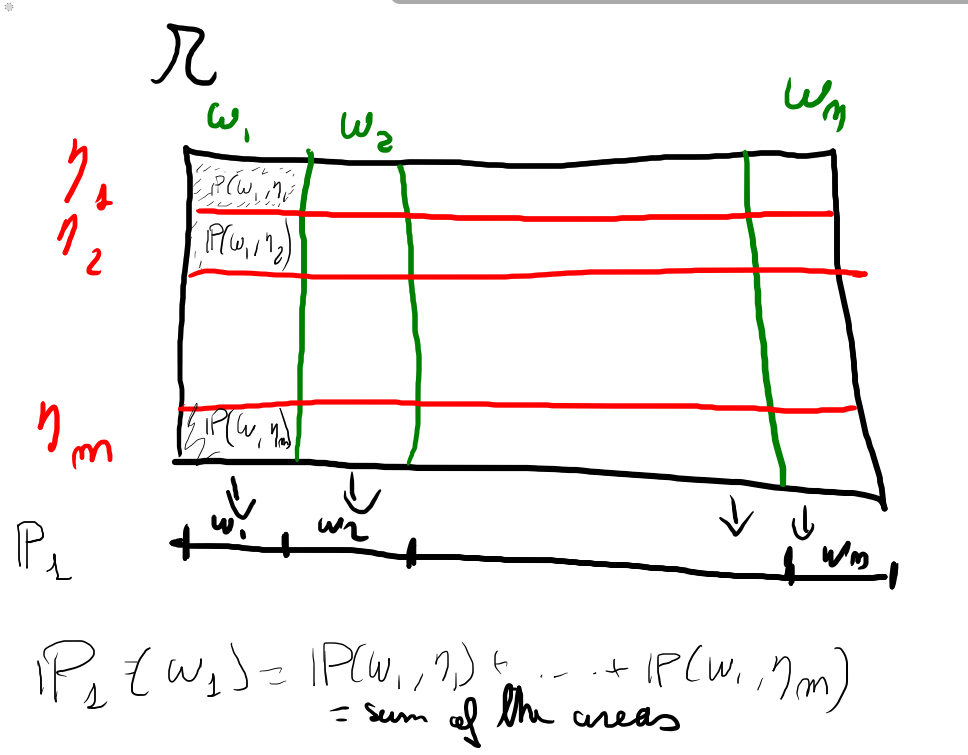
\includegraphics[width = 11cm]{Marginal.png}
\label{f:marginal}
\end{figure}
\begin{figure}[h]
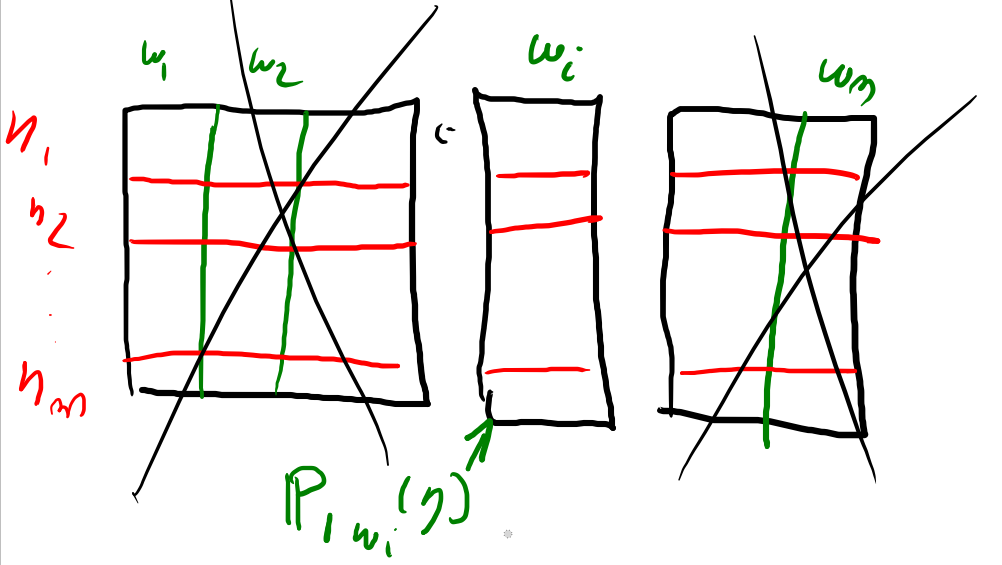
\includegraphics[width = 11cm]{conditional_graphical.png}
\label{f:conditional}
\end{figure}

\begin{ExerciseList}

\Exercise
On $\Omega=\{0,1\}\times\{0,1\}$ with probability $\mathbb{P}$ defined by
\bel{}{\mathbb{P}(0,0)=(1-q)(1-p)\,\,,\,\,\,\mathbb{P}(0,1)=(1-p)q,\\ \mathbb{P}(1,0)=p(1-q),\,\,\,\mathbb{P}(1,1)=pq,}
find the marginals of $\mathbb{P}$.
    
\Exercise Look at the examples at the beginning of this section, where the joint probability of the two coin tosses was defined by 
$\mathbb{P}(00)=\mathbb{P}(11)=1/2$ for the first glued coins,  $\mathbb{P}(01)=\mathbb{P}(10)=1/2$ for the second glued coins, $\mathbb{P}(ij)= 1/4$ for all $ij\in\Omega$ for the independent coins)

\Exercise Consider on $\Omega=\{(r,r),(r,b),(r,g), (b,r),(b,b),(b,g),(g,r),(g,b),(g,g)\}=\{(r,b,g)\}\times\{(r,b,g)\}$ the probability 
\bel{}{\mathbb{P}((b,b))=\mathbb{P}((g,g)) = \mathbb{P}((r,r))=0,} and $1/6$ for the other elementary events.  Calculate the marginal over $\Omega_2$, $\mathbb{P}_2$ (This is the probability of the second extraction).
Repeat the exercise with the uniform probability $\mathbb{Q}$ on $\Omega$.

\Exercise Compute the conditional probabilities of the systems described in the previous exercises. 

\end{ExerciseList}

Using the formula $\mathbb P(\omega,\eta) = \mathbb P(F_\omega S_\eta) = \mathbb P(\eta |\omega)\mathbb P(\omega)$\sidenote{This formula has the intuitive meaning that first we look at the first system and, knowing the first one we look at the second}, it becomes intuitive that the it suffices to know $\mathbb P_1$ and $\mathbb P_{|\omega}$ for each $\omega \in \Omega_1$ in order to define $\mathbb P$. This fact is the object of Proposition ~\ref{p:recovery}, let's show that the dimensionality are correct. If we know $\mathbb P_1$ we know $n-1$ numbers, and if we know $\mathbb P_\omega$ we kn know m-1 numbers for each $\omega \in \Omega_1$. We thus know $n-1 + n(m-1) = nm-1$ numbers, which are those required to kno $\mathbb P$.
\begin{proposition}
\label{p:recovery}

Let $\mathbb Q$ be a probability on $\Omega_1$ and $\mathbb Q_\omega$ be, for each $\omega \in\Omega$ a probability on $\Omega_2$. Then the formula
\bel{}{
    \mathbb P(\omega,\eta) = \mathbb Q_\omega(\eta) \mathbb Q(\omega)
}
defines a probability on $\Omega$. Moreover it's first marginal $\mathbb P_1$ coincides with $\mathbb Q$ and the conditional probabilities $\mathbb P_{|\omega}$ coincide with $\mathbb Q_\omega$. That is, 
\bel{}{
\mathbb P_1 &= \mathbb Q\\
\mathbb P_{|\omega} & = \mathbb Q_\omega \,\,\,\,\textrm{for each $\omega \in \Omega_1$.}
}
\end{proposition}

\begin{proof}
Let's first check that $\mathbb P$ is a probability. It is immediate to see that $\mathbb P(\omega,\eta)$ is a positive number and the fact that they are less that 1 will follow by showing that equality \eqref{e:fun} is satisfied, since if the sum of positive numbers is 1, then any of the numbers cannot exceed 1. Let's thus check \eqref{e:fun}
\bel{}{
    \sum_{i=1,...,n,j  = 1,...,m}\mathbb P(\omega_i,\eta_j) & = \sum_{i=1,...,n,j = 1,...,m}
    \mathbb Q_{\omega_i}(\eta_j) \mathbb Q(\omega_i) \\
    & = \sum_{i=1,...,n} \left(\sum_{j=1,...,m} \mathbb Q_{\omega_i}(\eta_j)\right)\mathbb Q(\omega_i)\\
     & = \mathbb \sum_{i=1,...,n} \mathbb Q(\omega_i) = 1,}
where on the last two steps I have used that $\mathbb Q_\omega$ and $\mathbb Q$ satisfy \eqref{e:fun}. Thus $\mathbb P$ defines a probability, and to check that the first marginal is the right one we simply compute 
\bel{}{
    \mathbb P(F_\omega) &= \mathbb P(\omega,\eta_1) + ...+ \mathbb P(\omega,\eta_m) = \mathbb Q_\omega(\eta_1)\mathbb Q(\omega) + \ldots + \mathbb Q_\omega (\eta_m ) \mathbb Q (\omega)\\
    & =\mathbb Q(\omega)\left( \mathbb Q_\omega(\eta_1) +...+ \mathbb Q_\omega(\eta_m) )\right) = \mathbb Q(\omega),}
as we wanted to prove. As for the conditional probabilities,
\bel{}{\mathbb P_{|\omega}(\eta) = \mathbb P(S_\eta | F_\omega) = \frac{\mathbb P(\omega,\eta)}{\mathbb P(\omega)} =\frac{ \mathbb Q(\omega)\mathbb Q_{\omega}(\eta)}{\mathbb Q(\omega)} = \mathbb Q_\omega(\eta),}
which concludes the proof. 
    \end{proof}



As we have seen in Subsection ~\ref{ss:examples}, the above Proposition is useful to build the probability measure $\mathbb P$. 

\subsection{Independent experiments}
\label{ss:indep}
When you regard that from the knowledge of the first experiment you cannot infer anything which changes the probabilities of the second one, you are making the following assumption $\mathbb{P}(S_{\eta}|F_{\omega})= \mathbb{P}(\eta_j)$, that is, we are taking $\mathbb P_{|\omega}(\eta) = \mathbb P(\eta)$ for all $\omega \in \Omega$. In this case 
In this case $\mathbb{P}(\omega_i,\eta_j) = \mathbb{P}(\omega_i)\mathbb{P}(\eta_j) = \mathbb{P}_1(\omega_i) \mathbb{P}_2(\eta_j)$, so that $\mathbb{P}$ is simply the product of the probabilities of the two experiments.  Note that independence has to be regarded as an hypotheses on the probability $\mathbb{P}(\eta_j | \omega_i) $ and you cannot tell whether it is or it is not true a priori: it is a property or an assumptions you  are making on the probability that you are assigning on $\Omega$. As Exercise \ref{ex:indep} shows, independence is much more general than causality (which is a property of events, not of probabilities) 

\begin{definition}
We say that the two experiments are independent if \bel{e:indexp}{\mathbb{P}(\omega_i,\eta_j)=\mathbb{P}("\omega_i \textrm{happens}")\mathbb{P}("\eta_j" happens)=\mathbb{P}_1(\omega_i)\mathbb{P}_2(\eta_j).}
\end{definition}

\begin{example} the sample space for the roll of a die is $\Omega=\{1,...6\}$. It is natural to put the uniform probability to each roll of the die, that is $\mathbb{P}(1)=...=\mathbb{P}(6)=1/6$. Why did we use the uniform probability on the outcomes of the roll of two dice? In this case $\Omega=\{(1,1),(1,2),...,(6,6)\}$. The fact is that the two rolls are independent:
\bel{e:uniform}{\mathbb{P}(i,j)=\mathbb{P}(i)\mathbb{P}(j)=1/36\,\,\,\textrm{ for every } i,j=1,..,6.}
This is precisely the uniform probability on $\Omega$.

\end{example}

\begin{ExerciseList}
\Exercise Assume that two experiments $\Omega_1=\{\omega_1,...,\omega_n\}$ $\Omega_2=\{\eta_1,...,\eta_m\}$ have the uniform probability (let $\mathbb{P}_i$ denote the uniform probability of $\Omega_i$). Show that, if they are independent, then the joint experiment $\Omega=\Omega_1\times\Omega_2$ have the uniform probability.
%\Answer  
%\bel{}{\mathbb{P}(\omega_i,\eta_j)=\mathbb{P}_1(\omega_i)\mathbb{P}_2(\eta_j)=\frac{1}{n}\frac{1}{m}}
%Since the number of elements in $\Omega$ is $m\cdot n$, this is precisely the uniform probability.
\end{ExerciseList}

\subsection{ Extractions}
We are now able to discuss rigorously the probability distribution of two extractions. 

\begin{ExerciseList}

\Exercise In an urn there are 4 red balls and 2 blue balls. We draw a ball, we reinsert it and then, independently from the first draw, we draw another ball. What is the probability of drawing balls of different color? 

\Exercise  There are $8$ lottery tickets, and each one of them is winning with probability $1/8$ \emph{independently} from the others. You buy $3$ tickets. What is the probability that at least one of them is winning.  Hint: consider the complementary event and use the independence. 

\Exercise There are $8$ lottery tickets, $4$ of which are winning. You buy $3$ tickets. What is the probability that at least one of them is winning.  Hint: consider the complementary event and
define the number \bel{}{X_i=\begin{cases}
1 & \textrm{if i-th first ticket is losing }\\
0 & \textrm{ if the i-th ticket is winning}.
\end{cases}
} for $i=1,2,3$. Using formula \eqref{e:chain} you should be able to calculate $\mathbb{P}(X_1=1,X_2=1,X_3=1)$.

%\Answer We need to compute the probability of the event A=" At least one ticket is winning". Consider the event $A^c$=" All the tickets are losing". We can proceed as follows: number your tickets from $1$ to $r$. Denote  
%\bel{}{X_i=\begin{cases}
%1 & \textrm{if i-th first ticket is losing }\\
%The event $A^c$ is the event $(X_1=1,...,X_r=r)$. We are therefore in the situation of the Bernoulli trials and we can use formula \eqref{e:chain} and write 
%\bel{}{\mathbb{P}(X_1=1,...,X_r=1)=\mathbb{P}(X_r=1|X_{r-1}=1,...,X_1=1)...\mathbb{P}(X_2=1|X_1=1)\mathbb{P}(X_1=1).}
%We now need to observe that the $\mathbb{P}(X_k=1|X_{k-1}=1...X_1=1)=(n-m-(k-1))/n-(k-1)$, since knowing that the tickets 1,...k-1 are losing, there are left  $n-(k-1)$ tickets, of which  $n-m-(k-1)$ are losing. Thus
%\bel{}{\mathbb{P}(A)=1-\mathbb{P}(A^c)=1-\frac{(n-m)(n-m-1)...(n-m-(r-1))}{n(n-1)...(n-(r-1)).}}

\end{ExerciseList}

